% This is "sig-alternate.tex" V2.1 April 2013
% This file should be compiled with V2.5 of "sig-alternate.cls" May 2012
%
% This example file demonstrates the use of the 'sig-alternate.cls'
% V2.5 LaTeX2e document class file. It is for those submitting
% articles to ACM Conference Proceedings WHO DO NOT WISH TO
% STRICTLY ADHERE TO THE SIGS (PUBS-BOARD-ENDORSED) STYLE.
% The 'sig-alternate.cls' file will produce a similar-looking,
% albeit, 'tighter' paper resulting in, invariably, fewer pages.
%
% ----------------------------------------------------------------------------------------------------------------
% This .tex file (and associated .cls V2.5) produces:
%       1) The Permission Statement
%       2) The Conference (location) Info information
%       3) The Copyright Line with ACM data
%       4) NO page numbers
%
% as against the acm_proc_article-sp.cls file which
% DOES NOT produce 1) thru' 3) above.
%
% Using 'sig-alternate.cls' you have control, however, from within
% the source .tex file, over both the CopyrightYear
% (defaulted to 200X) and the ACM Copyright Data
% (defaulted to X-XXXXX-XX-X/XX/XX).
% e.g.
% \CopyrightYear{2007} will cause 2007 to appear in the copyright line.
% \crdata{0-12345-67-8/90/12} will cause 0-12345-67-8/90/12 to appear in the copyright line.
%
% ---------------------------------------------------------------------------------------------------------------
% This .tex source is an example which *does* use
% the .bib file (from which the .bbl file % is produced).
% REMEMBER HOWEVER: After having produced the .bbl file,
% and prior to final submission, you *NEED* to 'insert'
% your .bbl file into your source .tex file so as to provide
% ONE 'self-contained' source file.
%
% ================= IF YOU HAVE QUESTIONS =======================
% Questions regarding the SIGS styles, SIGS policies and
% procedures, Conferences etc. should be sent to
% Adrienne Griscti (griscti@acm.org)
%
% Technical questions _only_ to
% Gerald Murray (murray@hq.acm.org)
% ===============================================================
%
% For tracking purposes - this is V2.0 - May 2012

\documentclass{sig-alternate-05-2015}
\usepackage{listings}
\usepackage{graphicx}

\begin{document}

% Copyright
%\setcopyright{acmlicensed}
%\setcopyright{rightsretained}
%\setcopyright{usgov}
%\setcopyright{usgovmixed}
%\setcopyright{cagov}
%\setcopyright{cagovmixed}
%
% --- Author Metadata here ---

%\CopyrightYear{2007} % Allows default copyright year (20XX) to be over-ridden - IF NEED BE.
%\crdata{0-12345-67-8/90/01}  % Allows default copyright data (0-89791-88-6/97/05) to be over-ridden - IF NEED BE.
% --- End of Author Metadata ---

\title{Final Project: Cell Processors}
\subtitle{ECE 568: Advanced Microprocessor Architecture, Spring 2016}
%
% You need the command \numberofauthors to handle the 'placement
% and alignment' of the authors beneath the title.
%
% For aesthetic reasons, we recommend 'three authors at a time'
% i.e. three 'name/affiliation blocks' be placed beneath the title.
%
% NOTE: You are NOT restricted in how many 'rows' of
% "name/affiliations" may appear. We just ask that you restrict
% the number of 'columns' to three.
%
% Because of the available 'opening page real-estate'
% we ask you to refrain from putting more than six authors
% (two rows with three columns) beneath the article title.
% More than six makes the first-page appear very cluttered indeed.
%
% Use the \alignauthor commands to handle the names
% and affiliations for an 'aesthetic maximum' of six authors.
% Add names, affiliations, addresses for
% the seventh etc. author(s) as the argument for the
% \additionalauthors command.
% These 'additional authors' will be output/set for you
% without further effort on your part as the last section in
% the body of your article BEFORE References or any Appendices.

\numberofauthors{2} %  in this sample file, there are a *total*
% of EIGHT authors. SIX appear on the 'first-page' (for formatting
% reasons) and the remaining two appear in the \additionalauthors section.
%
\author{
% You can go ahead and credit any number of authors here,
% e.g. one 'row of three' or two rows (consisting of one row of three
% and a second row of one, two or three).
%
% The command \alignauthor (no curly braces needed) should
% precede each author name, affiliation/snail-mail address and
% e-mail address. Additionally, tag each line of
% affiliation/address with \affaddr, and tag the
% e-mail address with \email.
%
% 1st. author
\alignauthor
Anthony Gallotta
       \email{agallo4@uic.edu}
\alignauthor
Vishal Mishra
       \email{vmishr2@uic.edu}
}
% There's nothing stopping you putting the seventh, eighth, etc.
% author on the opening page (as the 'third row') but we ask,
% for aesthetic reasons that you place these 'additional authors'
% in the \additional authors block, viz.
\date{24 April 2016}
% Just remember to make sure that the TOTAL number of authors
% is the number that will appear on the first page PLUS the
% number that will appear in the \additionalauthors section.

\maketitle
\begin{abstract}
In September 2006, IBM released its first implementation of the Cell Broadband Processor architecture, the first commercial heterogeneous CPU architecture. While originally designed for the PlayStation 3, the Cell quickly gained popularity in the scientific and high performance computing (HPC) communities thanks to its impressive performance in single precision (SP) floating point computations, low power consumption, and low cost. Several of the top performing supercomputers of the late 2000s utilized the Cell extensively as well. IBM released a 2nd implementation of the Cell architecture, the PowerXCell 8i, in 2008, but this became obsolete quickly, and in 2009 they announced that the Cell line would be discontinued. While most people subjectively agree that the Cell became obsolete due to the rise of GPUs, to the authors' knowledge there have been no studies directly comparing Cell performance to GPUs manufactured at the same technology scale, and with similar power and area budgets. This paper attempts to quantify the reasons the Cell architecture is no longer being produced, in terms of performance per Watt. In addition, we discuss some of the architectural principles that have lived on, those that haven't, and why. To do this, we create several models that resemble the Cell architecture. We model an architecture similar to the Cell using GPU cores that resemble the Cell SPEs, and model the memory structure of the Cell. We compare the performance of our model to that of a commercial GPU. We also construct a power and area model for the Cell in order to speculate on how the Cell architecture could have scaled beyond 45nm technology, and how it might compare to GPUs on the same scale.
\end{abstract}

\section{Introduction}
With a 4 year and \$400 million budget, Sony teamed up with IBM and Toshiba around 2000 to form STI, a group whose goal was to design a new processor for the PlayStation 3, targeting a performance improvement of at least 100x over the PlayStation 2 \cite{kahle2005introduction}. With a gaming system as its primary target, the main objectives for the processor were to support high performance on multimedia applications, real time user and network responsiveness, and to be able to apply the architecture to other systems, having a lifetime beyond a single gaming system. The biggest hurdles in achieving these objectives were expected to be memory speed and power constraints. After evaluating several design options, the developers decided that the chip would have one larger core based on IBM's Power Architecture, and a number of low power "synergistic" processors with simple architectures and SIMD instruction sets.
IBM released 2 implementations of the Cell architecture, the first of which was the Cell Broadband Engine (BE), built on a 90nm scale and used in the PlayStation 3. IBM introduced a second and final implementation of the Cell architecture specifically for their Roadrunner supercomputer, the PowerXCell 8i, which has enhancements to the DP pipeline allowing peak performance of up to 108.8 GFLOPs/s, a 7x improvement over the Cell BE \cite{barker2008entering}. This was a much needed improvement for HPC applications, however it didn't come until 2 years after the initial introduction of the Cell, and by this time GPGPUs were emerging as another option for HPC. The PowerXCell 8i also has support for up to 32GB of memory compared to the Cell BE's limitation of 2GB, but is largely unchanged other than these factors and the smaller 65nm process \cite{barker2008entering}. 
Thanks to its low cost in terms of both purchase price and power, the Cell quickly gained popularity in the HPC community. This is evident from supercomputers like the U.S. Air Force's Condor \cite{luley2011energy} that used a mix of Cell, GPU, and homogeneous multicore processors, and IBM's Roadrunner \cite{barker2008entering} that primarily uses PowerXCell 8i cores, with support from Opteron cores for coordination.

\section{Background}

\subsection{Cell Architecture}
The architecture for the Cell is called the Broadband Processor Architecture, although the term "Cell" is commonly used to refer to either the architecture, or an implementation of the architecture, depending on the context. The Cell is a heterogeneous architecture that consists of a single large core, the "Power Processing Element" (PPE), and many smaller, SIMD cores, the "Synergistic Processing Elements" (SPEs). This section focuses on high level architecture components, such as the cores themselves, memory hierarchy, and interconnects. It is noteworthy though, that no detail was neglected in the first Cell implementation. Hardware components were optimized all the way down to the gate level for the first generation of the Cell. Along with other components, STI developed several custom latches and flip flops to improve power efficiency and delay, and observed correct operation at frequencies approaching 5GHz \cite{pham2005design}.

\subsection{Power Processing Element}

The PPE is a dual-threaded, dual-issue (in order) 64-bit Power Architecture compliant core. This processor has a traditional cache hierarchy and 2 hardware threads. In typical HPC implementations it is used only to control the 8 synergistic processing elements (SPEs) and run an operating system, however it can also be used to run applications that have not been updated to utilize the SPEs, are highly serial, contain complex control flow logic, or are otherwise not suitable for execution on the SPEs.

\subsection{Synergistic Processing Elements}

Each SPE has direct memory access (DMA) to main memory, and a fast local memory, as well as a large 128 register file. All 8 SPEs are connected via a 25.6 GB/s element interconnect bus (EIB), which also provides connections to main memory and I/O controllers \cite{kahle2005introduction}. A SIMD instruction set (with scalar support) was chosen for the SPE, as it had become the dominant ISA for CPU media support at the time, and it is optimized for power and performance on media and compute-intensive operations.
The largest component in the SPE is the local store (implemented with SRAM), which is where the unit loads data and instructions from, and what differentiates the Cell architecture most from traditional cores that use an L1 cache. An SPE issues DMA commands (up to 16 may be outstanding) in order to load data from main memory (or another SPE core, if it has permission) to its local store. Since the local store must be explicitly managed by software, memory latency is constant, compared to a hardware managed cache, where it is unknown to the programmer what may be in the various cache levels at any given time. While this adds some programming complexity, it also results in more predictable performance, and lower power consumption. This generally results in a much higher memory bandwidth as well, since the software is able to load more useful data then a cache. Branch prediction logic is lacking in the hardware layer, with only a simple static predictor, and must be implemented in software if a better predictor is desired \cite{flachs2006microarchitecture}. Mispredicted branches can be costly as well, with a pipeline flush requiring 18 cycles, so software should be cautious of this. This simplicity again results in higher area and power efficiency. The SPE is an in order processor, and does not perform any register renaming, although it can issue two instructions per cycle if execution units are available for both.

\section{Related Work}

Numerous studies have been published [4,5,6] comparing the performance of the Cell to homogeneous and single core architectures. In \cite{chen2007cell}, published by IBM, the authors compare performance of scientific applications on the Cell against competitive superscalar and SIMD architectures and demonstrate its superiority to both, but GPUs are not considered.
In \cite{hofstee2005power}, an article published by IBM before the first release of the Cell BE, the authors explore performance per transistor as an efficiency metric. This metric approximates performance per Watt, assuming a constant power draw per transistor, which is reasonable to make under CMOS technology \cite{hofstee2005power}. They detail the design trends of architectures that tend to decrease this efficiency, and advocate architectural details like the local store used in the Cell to improve performance per transistor. While all of their logic makes sense intuitively, the authors fail to quantify any of their statements with experimental results.
High performance LINPACK (HPL) is a benchmark that solves a dense system of linear equations, and is commonly used to measure performance of supercomputers for rankings such as the TOP500 \cite{about_hpl} and Green 500 \cite{green500}. The U.S. Air Force's Condor Cluster was designed to be competitive with top supercomputers in terms of raw performance, but with much greater energy efficiency. It's target applications were also optimized to use SP computations. To achieve its goals, the system was designed to have 78 compute nodes, each composed of 2 NVIDIA GPGPUs, 1 Intel Xeon X5650 (a 12 core chip), and a connected subcluster of 22 PS3s. In \cite{luley2011energy}, the authors run HPL on a cluster of 2 PS3s and calculate an energy efficiency of 52 MFLOPS/W, which is sufficient to place the PS3 nodes of the Condor in the top 20\% of the November 2010 Green 500 List. The authors report the same metric for the NVIDIA C2050 nodes, which obtain an energy efficiency of .966 GFLOPS/W, which would place them in the top 99\% of the same list. The authors do not make the comparison here since it is not the focus of their research, we can extrapolate these results to make some comparisons between the Cell and GPU. This is not the PS3's best possible performance since the HPL implementation uses double precision (DP) floating point computations. If we assume the same power consumption (199W average) and the improved DP performance of the PowerXCell 8i of 108.8GFLOPS, we can roughly calculate a best case performance for the Cell architecture of 0.547 GFLOPS/W, which is still just better than half the efficiency of the GPU. There are some flaws in this calculation, such as the fact that the PS3 used in \cite{luley2011energy} used a Cell chip manufactured using a 90nm technology, versus the 40nm \cite{techpowerup} process used for the GPU, but it gives direction for future comparisons.
Cell based systems remained near the top of the Green500 list from 2008 to 2010. The June 2010 Green500 list \cite{green500_062010} reports a PowerXCell 8i cluster in position \#1, achieving 773 MFLOP/s, the last time a Cell based system topped the list. From November 2010 onwards, the Cell systems were surpassed by both homogeneous multicore and GPU based systems. 

\section{Methodology}

In order to predict how the Cell architecture may have evolved, and level the playing field for comparison with modern architectures, we construct models for performance, power, and area of the Cell.

\subsection{Performance Modeling}
When the Cell was still in production, IBM provided a full system simulator for the architecture. They have since removed all download links from their website, and no longer offer any kind of support for the tool. We were able to find a copy of the simulator from another source, and eventually run the simulator on a virtual machine running Fedora 23. However, we found that the simulator would only be capable of running Fedora 7, or no operating system, which would make it difficult for us to compile and execute modern benchmarks on the simulator. Furthermore, we were unable to find a copy of the Cell SDK that would be required to compile programs to execute on the simulator, as IBM no longer makes this available either, so we would have needed to find benchmark binaries already compiled for the Cell to run. Due to all of these factors, we decided the Cell system simulator would not be feasible for use in our study.

To simulate and model our Cell processor we used the Multi2sim simulator \cite{multi2sim}. It simulates various instruction set architectures like x86, ARM, AMD Evergreen, AMD Southern Islands and Nvidia's CUDA. It provides statistics on performance based on the execution of a program. For our study, we have focused on the detailed simulation feature provided with the multi2sim. It is a timing or architectural simulator, that is, the software component models hardware structures and keeps track of their access times. The modeled hardware includes pipeline stages, pipe registers, instruction queues, functional units, cache memories and others. The program is broken up into instructions and a pipeline model is created where ISA like execution is mimicked by the simulator. 

In our study we focused on the application only emulation rather than the full system emulation. This choice is made since we work on understanding the working of cell processors and also compare it to the Graphics processors. Since application level changes needed to be implemented in order for the program to take benefit of the architecture. With IBM introducing APIs for programmers where they can  leverage branch prediction and memory management in their programs. 

Although Multi2sim does not support IBM's Power Instruction set Architecture, we have made an informed choice to see the comparison between cell architecture and GPU architectures in terms of performance, by focusing on the architectural aspect that distinguishes the Cell architecture most from traditional CPUs and GPUs: the local storage. So for our study, we use the x86 Instruction Set Architecture (ISA) for the larger PPE-like core and AMD's Southern Islands ISA for the SPE like cores, as well as the GPU cores. This enables us to perform a fair comparison evaluating only the impact of using local storage over a cache. Once we have the common base configuration set, we can then focus on creating a similar architecture for cell processor and GPUs. 

\subsection{Power/Area Modeling}

For power and area simulation, we use McPAT(Multicore Power, Area, and Timing) \cite{li2009mcpat}. McPAT allows for configuration of many processor components and parameters, from general parameters like clock frequency and transistor size to component level details like cache line size and associativity, integer and floating point pipeline lengths, etc. For the SPE cores, we build off the sample configuration McPAT provides for the Niagara architecture. We felt this was a good starting point as this architecture is similar to the Cell in the sense that it seeks to achieve low power per core, and prefers a large number of simple in-order cores over complex superscalars. We substitute all of the published Cell parameters that we can find into this configuration, leaving the rest unmodified. A similar process is used for the PPE core, borrowing some of the baseline parameters from the Intel Xeon configuration provided with McPAT. This is similar to the methodology used in \cite{pham2005design} to simulate a GPU using McPAT.

Our model does have some inherent flaws, however, since we are limited to the capabilities of McPAT. Although the Cell architecture features 7 specialized execution units for integer and floating point operations per SPE \cite{flachs2006microarchitecture}, McPAT does not allow for this level of detail in its component modeling, so we simply tune these parameters such that they occupy a similar fraction of area. An SPE contains two pipelines, which can be modeled in McPAT, however this does not completely reflect the SPE architecture, as McPAT only allows separate integer and FP pipelines to be configured, while the SPE has 1 mixed integer and FP pipeline \cite{flachs2006microarchitecture}. A slight consolation is made modeling the register file, where McPAT requires explicit modeling of integer versus FP registers, while the SPE has general purpose registers that can be used for either \cite{flachs2006microarchitecture}. Although the SPE contains a simple static branch predictor, we do not model this because McPAT only includes a tournament style branch predictor. We find this an acceptable omission considering the branch predictor accounts for only 3\% of the SPE area. Unfortunately, McPAT does not provide for the possibility of a local memory instead of a cache. McPAT models the L1 cache as part of the instruction fetch unit, and the data cache as part of the load and store unit \cite{li2009mcpat}. Therefore, we compensate for the necessity of using a cache by adjusting the L1 parameters until the area of our modeled chip is comparable to its corresponding component in the Cell architecture. We label our model architecture "Cell\$" to indicate the addition of a cache. For area modeling, we believe this is a reasonable consolation to make since we are trading one memory structure for another. For power modeling, we will need to compensate for this differently, as the cache will surely consume more power than a local memory store would.

\begin{figure}
\centering
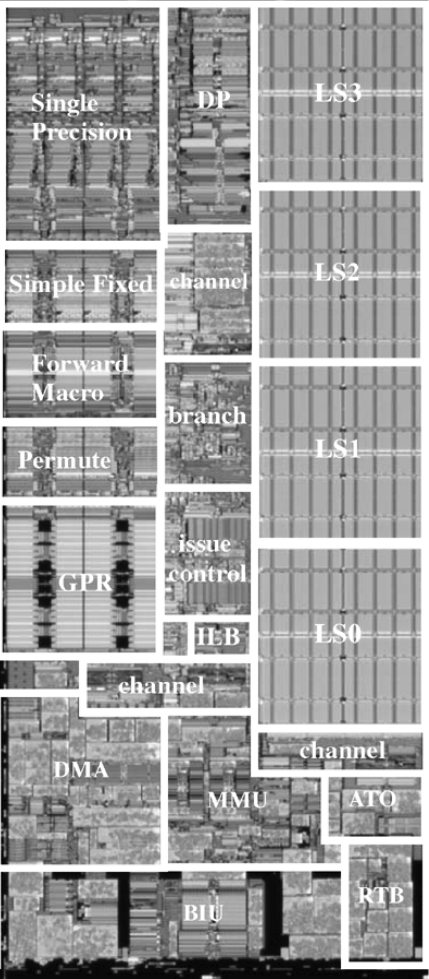
\includegraphics[scale=0.4]{./spe}
\caption{A photo of the SPE die}
\label{spe_die}
\end{figure}

\section{Experimental Results}

\begin{table*}[t]
\centering
\begin{tabular}{| l | c | l |} \hline
\# SPEs & Technology Scale (nm) & Peak Power (W) \\ \hline
8 & 90 & 146 \\ \hline  
8 & 45 & 51 \\ \hline  
8 & 28 & 19 \\ \hline  
16 & 45 & 89 \\ \hline  
16 & 28 & 33 \\ \hline  
32 & 45 & 165 \\ \hline  
32 & 28 & 60 \\ \hline  
\end{tabular}
\label{table:cell_model_power}
\caption{Cell model power by technology}
\end{table*}

\subsection{Area Model Validation}

The dimensions of the initial 90nm SOI technology SPE were 2.54mm by 5.81mm (14.76 $mm^2$), per \cite{flachs2006microarchitecture}. We use this as a target for our McPAT model. We use the image of a SPE provided in \cite{flachs2006microarchitecture}  and shown in figure 1 to calculate the percentage of the die occupied by each unit, based on the number of pixels it occupies, and compare this to our McPAT output. Overall, the Cell occupies an area of 221 $mm^2$ \cite{realworldtech} , while our model occupies 291 $mm^2$. McPAT provides output in terms of functional blocks within the core - categorizing all subcomponents as part of the instruction fetch unit (IFU), load-store unit (LSU), memory management unit (MMU), or execution unit (XU). For the total area of the core, it reports a number larger than the sum of these 4 units, so we categorize this area into "Others". \cite{li2009mcpat} details the subcomponents contained in many of these units. However, there are still some parts of figure \ref{spe_die} that we cannot determine a one to one mapping for. We intuitively categorize the local storage as part of the LSU, since this is where McPAT puts the L1 data cache, and we put the remainder into the "Others" category as this makes sense from the perspective of chip area allocation.

\subsection{Power Model Validation}

To validate our power model, we compare our model SPE's power consumption to the voltage/frequency shmoo published for an SPE in \cite{flachs2006microarchitecture}, both at 90nm. The published results we compare to are integer values only, which makes it difficult to judge the trend. We see that in the worst case, our model consumes 3x the power of the actual SPE, and 2x at a higher voltage ($V_dd = 1.3$). We can attribute this to several factors. First, our model uses a cache, which we know to draw more power than the local storage used in an SPE. Second, we know that STI designed several custom latches and latches \cite{pham2005design} to improve power efficiency and latency on the Cell, whereas McPAT has been validated against more commonly used hardware components. The results published in \cite{flachs2006microarchitecture} also note that they are reporting "active power", which they define as the amount of power consumed by switching logic and array circuits. While this sounds the same as the peak  power numbers we gather from McPAT, there may be some difference in the methodology of power reporting. Unfortunately it is quite difficult to find published TDP values for the entire Cell BE chip at 90nm. IBM has removed all Cell specifications from their site, however unofficial sources report TDP as high as 110W for the chip alone, and a peak of 199W has been observed for the PlayStation 3 running a 90nm Cell BE core, and powering other components such as a hard drive, etc, giving a high upper bound. Our model gives a peak power of 146W for the chip overall. Even with some uncertainty in the published SPE results, and inconsistent reports of overall TDP, it seems probable that our model is consuming more power than the actual Cell BE would.

To further evaluate the accuracy of our model, we compare a 45nm scale version to the PowerXCell8i, whose only significant architectural change other than SOI technology was the floating point pipeline. At 45nm, our model gives a peak power of 50W, which is significantly lower than the 92W TDP reported for the PowerXCell 8i in \cite{powerxcell}. This leads us to have some doubts in the validity of our model. Table \ref{table:cell_model_power} shows the peak power output from McPAT for different numbers of SPE cores in our model, and at different technology sizes. The power consumption appears to decrease at a rate faster than linear with technology scale. It is possible that the 45nm PowerXCell did not fully take advantage of technology improvements that McPAT is modeling at this scale, but this still leads us to be skeptical that the McPAT power levels would actually be attainable. Taken at face value, these results do give some hope for the theoretical scalability of the Cell architecture, as far as its ability to remain power efficient.

\subsection{Energy Efficiency vs. Modern GPU}

We compare our Cell models to a modern GPU architecture. The AMD Radeon 7970 is an ideal candidate, as an example configuration is provided with Multi2Sim that has been validated against this architecture, and AMD has published results on its theoretical peak performance and power consumption. Released in 2012, the Radeon 7970 was built using a 28nm process, has a peak theoretical DP performance of over 1 TFLOPS, and a peak power draw of 250W \cite{radeon7970}. Therefore, it has a peak theoretical performance/power ratio of 4 GFLOPS/W. With a peak DP performance of 108.8 GFLOPS in the PowerXCell 8i, assuming we could scale this to 32 SPEs without running into further limitations, we would expect a peak theoretical DP performance of 435.2 GFLOPS on a 32 SPE Cell processor. For our 32 SPE Cell model, we quadruple all shared resources as well. We obtain a peak power consumption of 65 W, which using our theoretical peak performance gives a peak theoretical power efficiency of 6.7 GFLOPS/W. This result gives some hope that it may be possible for the Cell architecture to compete with GPGPUs, however, our performance modeling shows that the architecture cannot achieve anything near this peak theoretical performance.

\begin{table*}[t]
\centering
\begin{tabular}{| l | c | c | c | c | l |} \hline
\textbf{Category (McPAT)} & \textbf{Subcomponent} & \textbf{Cell (\%)} & \textbf{Cell ($mm^2$)} & \textbf{Cell\$ (\%)} & \textbf{Cell\$ ($mm^2$) }\\ \hline
\textbf{Instruction Fetch Unit}  & &  7.4\% & 1.09 & 10.0\% & 2.17 \\ \hline
  & Issue Control & 4.2\% & 0.61 & & \\ \hline
  & Branch Predictor & 3.2\% & 0.47  & & \\ \hline
\textbf{Load Store Unit}  & & 36.1\%  & 5.32 & 30.3\% & 6.58 \\ \hline
  & Local Storage & 29.2\% & 4.31 & & \\ \hline
  & DMA & 6.8\% & 1.01  & & \\ \hline  
\textbf{Memory Management Unit} &  & 6.8\% & 1.01 & 6.4\% & 1.39 \\ \hline
 &  MMU & 6.8\% & 1.01   & & \\ \hline  
\textbf{Execution Unit}  & & 29.4\% & 4.33 & 27.6\% & 6.01  \\ \hline
 & Floating Point & 13.8\% & 2.03      & & \\ \hline  
 &  Integer & 9.7\% & 1.44      & & \\ \hline  
 & Register File & 5.8\%  & 0.86      & & \\ \hline  
\textbf{Others} &  & 20.4\% & 3.01 & 25.8\% & 5.61  \\ \hline
 & Channels, etc. & 6.5\% & 0.96      & & \\ \hline  
 & Bus Interface Unit  & 9.4\%  & 1.39      & & \\ \hline  
 & Relational Translation Buffer & 4.5\% & 0.66      & & \\ \hline  
\textbf{Total}  & 100\%  & 14.75 & 100\% & 21.75   \\ \hline
\end{tabular}
\label{table:spe_area}
\caption{Cell model vs. actual area at 90nm}
\end{table*}

\begin{figure*}
\centering
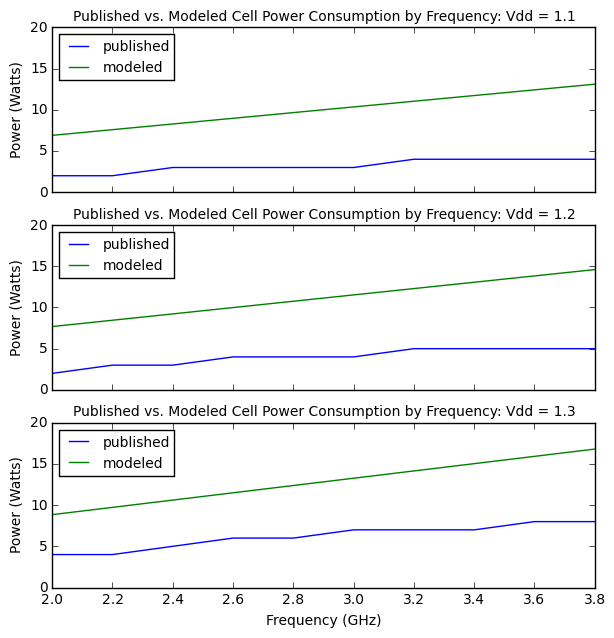
\includegraphics{./spe-voltage-freq}
\caption{Model vs. published power consumption for an SPE}
\label{spe-voltage-freq}
\end{figure*}

\subsection{Performance analysis}

To better understand how the architecture works and its eventual demise, we tried to replicate the processor in x86 based ISA. We did this in part due to the difficulty of finding a simulator for the Power ISA, and to rule out ISA differences among Cell processors and Graphics processing units as a factor in performance. To understand our analysis, we must think of the architecture of Cell processors and GPUs in the year 2009.  

IBM’s next planned line of cluster computing grade Cell Processors would have had 32 SPEs per chip. Comparing this to a GPU, we see a minimum of 32 Streaming processing threads on chip. This allows for a configuration where we can have one central processor to manage and give work to the other processing elements. Here we can single out the major portion of the processor. So using Multi2sim we create an architecture based on x86 ISA. With a base design in mind, we can proceed towards creating a similar configuration on Multi2sim. 

%<Config Screenshot image> 

Since, SPEs did not have caches in them, we have not included caches in their design. They however had a SRAM access which was slower than a cache but was available on chip. To mimic that we simulated the cell processor with adequate latency. All the SPEs can share a common SRAM-based on chip memory coupled with an interconnect network that would allow for high bandwidths. We use AMD’s graphics processor elements to mimic a Cell architecture. So all of the SPEs run a specialized Southern Islands ISA. The GPU model on the other hand has a Level one cache shared by a group of  8 of the streaming processors, and a Level 2 cache that is shared by all of the streaming processors. This is the difference between the two architectures on a level where everything else is normalized for our study. 

To model the PPE, a general purpose core responsible for executing scalar applicationsm, we included a standard x86 based architecture core. The use of a PPE core for our simulations, where no operating system is involved, is to provide the data computation for SPEs, which can execute parallel sections of the application much more efficiently. 

Lastly, we picked benchmark applications that were coded to take use of the SPE cores or the streaming cores (GPU). This allows the central processor to assign parallel jobs to the specialized units, and itself be responsible for executing scalar and managing the processes on the operating system.

Ideally we would have liked to use the industry standard unit of Floating point operations per second (FLOPS), however we were not able to get this output from Multi2Sim for our selected architectures. Since, our analysis is not just towards high performance or supercomputing, we will take a general view of performance to see where the Cell processor can be used and how it is out of the market now. For this, we use Operations (Instructions) per second (OPS) and Operations per second per Watt (OPS per Watt) as our units of measurements. All results are normalized such that the Cell model has a value of 1 for each measurement.

\begin{figure*}
\centering
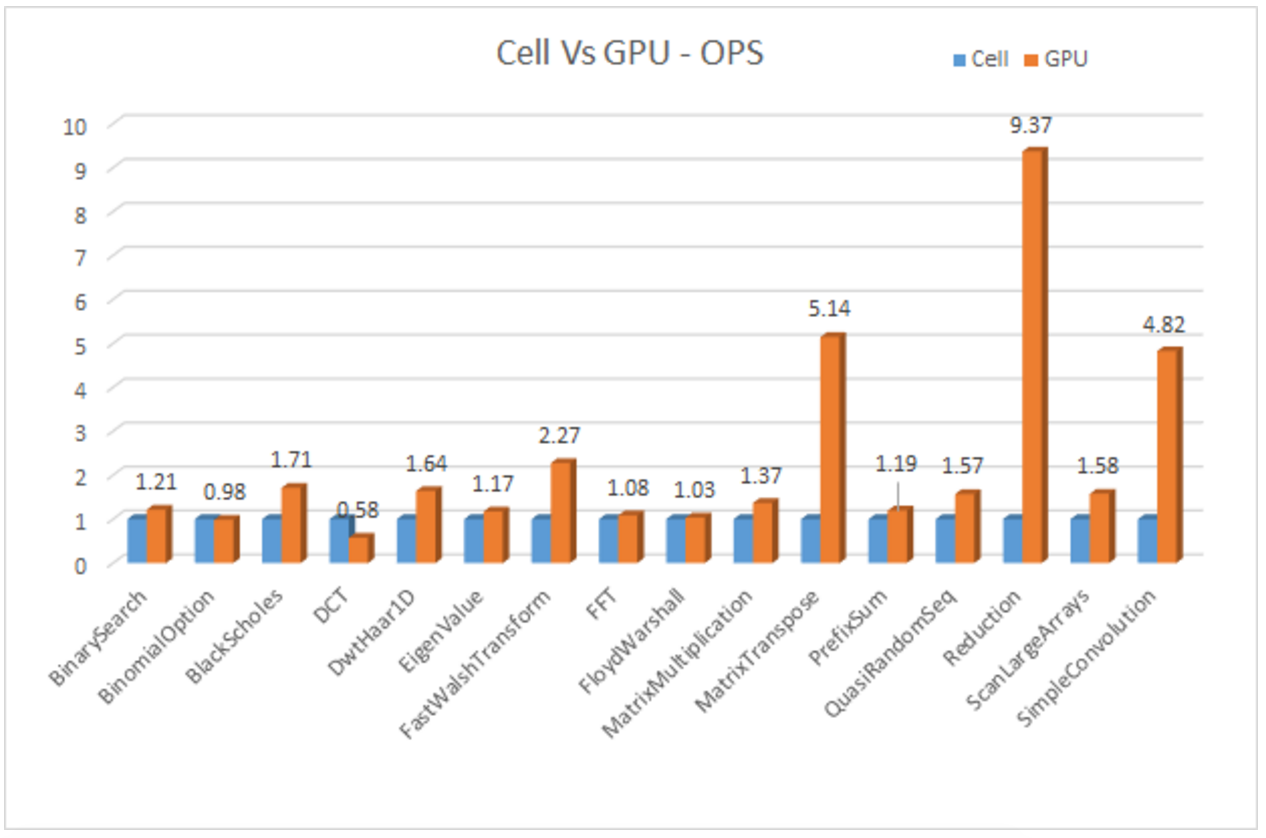
\includegraphics[scale=0.8]{./cell_gpu_ops}
\caption{Modeled Cell vs. GPU performance - normalized to 1 for Cell}
\label{cell_gpu_ops}

\centering
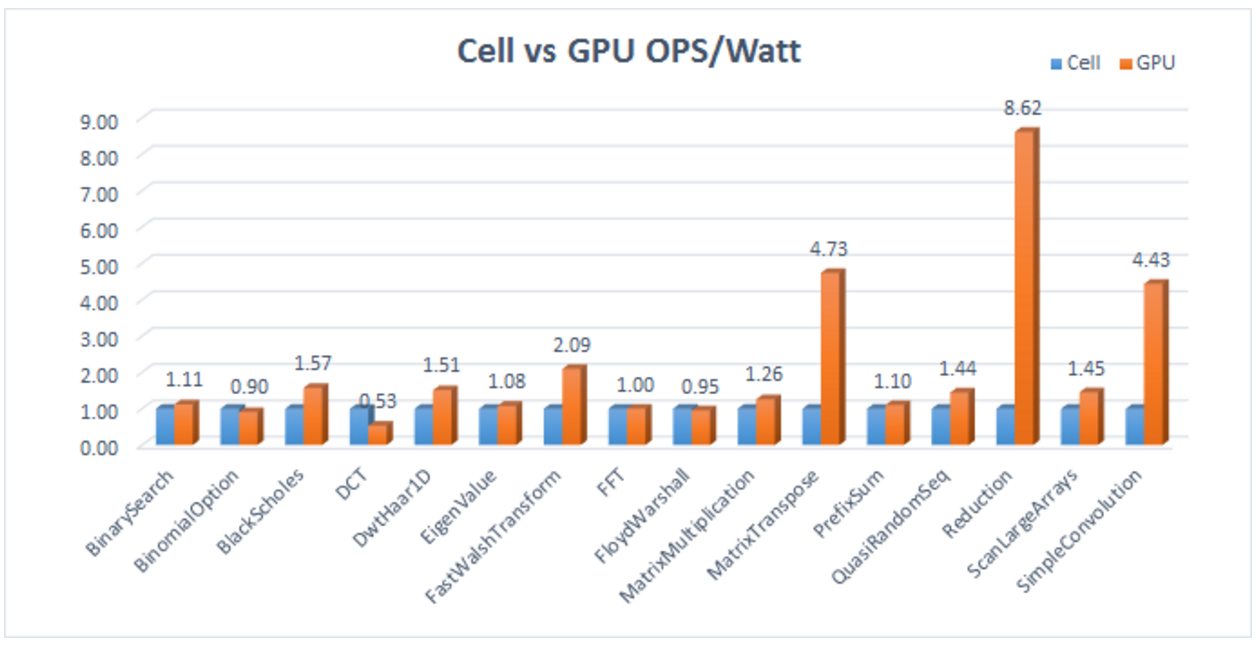
\includegraphics[scale=0.8]{./cell_gpu_opsperwatt}
\caption{Modeled Cell vs. GPU performance / power - normalized to 1 for Cell}
\label{cell_gpu_opsperwatt}
\end{figure*}


From figures \ref{cell_gpu_ops} and \ref{cell_gpu_opsperwatt} we see how much performance difference can be seen between Cell processors and GPUs. We ran through multiple parallelized computational applications to see how their underlying architectures govern their performance. 

First, we start our analysis to measure the peak performance capabilities (figure \ref{cell_gpu_ops}), for this reason we do not focus on power consumption.  Here we see for some programs the Cell processors performed almost as well as the GPU. There is only a marginal gain in performance in benchmark applications such as BinomialOption, FFT and FloydWarshall. This can be due to the low inherence cache requirement in these applications. So the performance of both the parallel applications is similar to each other in the different architecture. 

In other applications we can see a fair amount of performance gain when using GPUs. Cell processors we have taken for our study includes a 32 SPE configuration without a cache memory. So applications which are computationally heavy will tend to store more data in cache and get better performance out of it. Here we see Binary Search which is a fairly scalar method of computation doing better on GPUs but applications which are highly parallel like MatrixTranspose, FastWalshTransform, Reduction and SimpleConvolution use the benefits of caches and interconnects to perform significantly better than the cell. The GPU uses its Streaming processors along with its level 1 and level 2 caches to outperform in such applications. These applications have a tremendous amount of parallel segments in them, this can be utilized by the GPU architecture along with the programming APIs that help it to do so. 
The results here are conclusive enough to show how much of performance increase can be achieved by GPUs while the area and power constraints are kept same. 

Lastly, we shift our focus on the performance to power aspect of our analysis. Here we try to keep both of the architectures  at a similar scale and simulated them while keeping power into consideration. Traditionally, when IBM’s cell architecture was running supreme in supercomputers, they were featured as one of the most energy efficient processors made. So as a unit of measurement we use Operation per second per Watt. 

From figure \ref{cell_gpu_opsperwatt}, we can see if by including the power into our study, the cell architecture could perform close to the GPUs. Since we had low confidence in the scalability of our power model, and we were unable to directly model the local storage, the primary variable in our performance model, we once again use the published TDP for the AMD Radeon 7970. Our GPU is modeled after this architecture exactly, and our Cell model deviates from only in the sense of the memory hierarchy. For the GPU, we use the published value of 250W directly in the denominator for our OPS/Watt computations. For the Cell, we deduct 20W. To arrive at this amount, we looked at results of a slightly older GPU modeled in \ref{lim2014power}, where the authors saw a maximum power consumption of near 20W for the L1 and L2 caches combined. We take this to be an upper bound, since we know the local storage will consume a nonzero amount of power.

We can see for some applications Cell processors perform marginally better than the GPUs. In our analysis, cell processors takes less power due to the lack of caches and simple branch predictors. This is consistent in the simulation results we get. Even though this is true, GPU still performs better in most of the applications. Cell processor do well in applications which do not require it to use a cache. Since IBM provided API to programmers to manage memory and predict branches in code itself, it also provided compiler modifications to suit the parallel needs. Still with the introduction of thread level parallelism introduced by the GPU architecture, the progress in Cell architecture was nullified. We see that GPUs perform better even when we take power into consideration. Since only a small amount of power is taken extra by GPUs when compared with Cell processors, but they provide an exponential speedup. 


\bibliographystyle{abbrv}
\bibliography{sigproc}  % sigproc.bib is the name of the Bibliography in this case
%
% The following two commands are all you need in the
% initial runs of your .tex file to
% produce the bibliography for the citations in your paper.
%\bibliographystyle{abbrv}
%\bibliography{sigproc}  % sigproc.bib is the name of the Bibliography in this case
% You must have a proper ".bib" file
%  and remember to run:
% latex bibtex latex latex
% to resolve all references

\end{document}
